\documentclass[a4paper,11pt]{report}
\usepackage{graphicx}
\graphicspath{ {./img/} }

    \title{Asteria Project Documentation}
    \author{Albert van Kiel, Timo Hermsen, Robin Baneke,\\ Max van Hasselt, Robert Kleef and Menno Prinzhorn}
    \date{\today}
    
	\begin{document}
    
    \maketitle
    
    \chapter{Introduction}
	    
    During the course of this project, we are creating a free and open source framework that contains the generic algorithms and file handling for astronomical data sets. 
    This framework will be modular. Similar to OpenCV, wherein specific modules can be added and disabled depended on the needs of a project. 
    This framework will be implemented in Python and C++.
    
    \section{Current situation}
    
    The development of the application is split into multiple parts and distributed over two different teams, there are two teams on handling the in and output (team IO) and one implementing algorithms (team Algorithm). Each team is assigned to work on their own part of the 			    project, at the end of each sprint the parts will be merged together, the result will be delivered to the product owners.

    For the IO part the eScience Center is in need of an application that is able to both read and write filterbank files. There already is an application in use. 
    However, the current application is outdated and therefore has to be rewritten. The scope of this project is to rewrite a new software stack with updated technology, 
    such as using the GPU which is highly modular and re-usable.

	The Algorithm part will be developing an application that detects pulsars in large datasets. The pulsars will be detected using the fast fourier transformation. Also, since the datasets are very large, we might want to do a parallel computing implementation for the algorithm in the          	future.

    We are using Scrum as our project method. By applying Scrum we are able to make changes, based on the feedback given by our product owners, whenever necessary to the application.
    
    \chapter{Plan of action}
    
    \section{Mission}
    
    The purpose of the IO part of the project is to read and write filterbank files.

	For the Algorithm part of the project the goal is to detect pulsars in large datasets using algorithms.

	The solutions will first be implemented in Python and later in C++.
    
    \section{Monitoring performance}
    
    In order to monitor the performance of our development our product owners decided to plan weekly reviews. These reviews could be used to discuss the pace of our project. 
    If our product owners are not satisfied with the pace of our development team, we could look at possible improvements.
    
    \section{Risks}
    
    \begin{itemize}
        \item A shortage of knowledge about Python/C/C++
        \item An inflation of requirements
        \item A wrong estimation of required development time
        \item Lack of motivation
    \end{itemize}
    
    \chapter{Technical details}
    
    \section{Requirements}
    
    The requirements can be divided into two different categories. There are both functional and non-functional requirements.
    
    \subsection{Non-functional}
    
    The non-functional requirements describe the technical requirements for the application.
    
    Since some users might have problems understanding C++ code we will develop a standalone version in Python, since Python is readable even without a lot of programming knowledge.
	By doing this we give users the possibility to focus on the logic of the algorithm without needing C++ knowledge.
    
    \begin{itemize}
        \item Support for:\\ MacOS High Sierra (x86\_64), CentOS (x86\_64), Raspbian(ARM\ x64)
        \item Python 3.6
        \item C++ 14
        \item Must be modular
    \end{itemize}
    
    \subsection{Functional}

    All users:
	\begin{itemize}
        \item As user I want to read filterbank files in my program, so we can use the astronomical data in scientific programs.
        \item As user I want to write filterbank files in my program, so we can write astronomical data in scientific program
		\item As a user I want to downsample given input, so it can be used in a later stage.
		\item As user, I want clear exceptions when something is not set right, so i can more easily debug my program.
	\end{itemize}
	AUAS Students:
	\begin{itemize}
		\item As student I don't to worry about thread safety, so it's usable in highly threaded applications.
		\item As student I want that Asteria is easily imported, so I can easily import it in other projects.
		\item As a student, I want that Asteria runs on limited PC hardware, so I can test my projects on my personal computer.
    \end{itemize}
	Scientific programmer:
	\begin{itemize}
        \item As scientific programmer I want that my filterbank reader performs with very large datasets (+1TB of data), which is often the case in software
        \item As scientific programmer I want that my filterbank writer performs with very large datasets(+1TB of data), which is often the case in software
		\item As scientific programmer, I want to downsample large sizes the input time series(+1TB) so it can be used in astronomical projects.
    \end{itemize}    

    \section{Efficiency measurements}
    
    In this chapter we discuss the efficiency of the modules and its methods, by performing benchmarks and profiling and looking at the Big O of some methods.

    \subsection{Computional complexity}

    The complexity of the discrete Fourier transformation is equal to $O(n^2)$, and for the fast Fourier transformation the complexity is equal to $O(n\,log\,n)$.

    To test whether expected Big O holds true when running the actual methods, we decided to benchmark the different methods. The results of benchmarks are described
    and explained in the upcoming paragraph.

    \subsection{Benchmarks}
    
    Furthermore, we measured and compared running the discrete Fourier transformation with the fast Fourier transformation. For each method, we ran it using different sample sizes.
    After performing the measurements we noticed that while the time it took to run the discrete Fourier transformation increased almost quadratically, the time it took to run fast 
    Fourier transformation increased linearly. This difference in efficiency becomes increasingly important when running the pipeline using larger sample sizes.

    \begin{figure}[h]
        \hspace*{-2cm}                                                           
        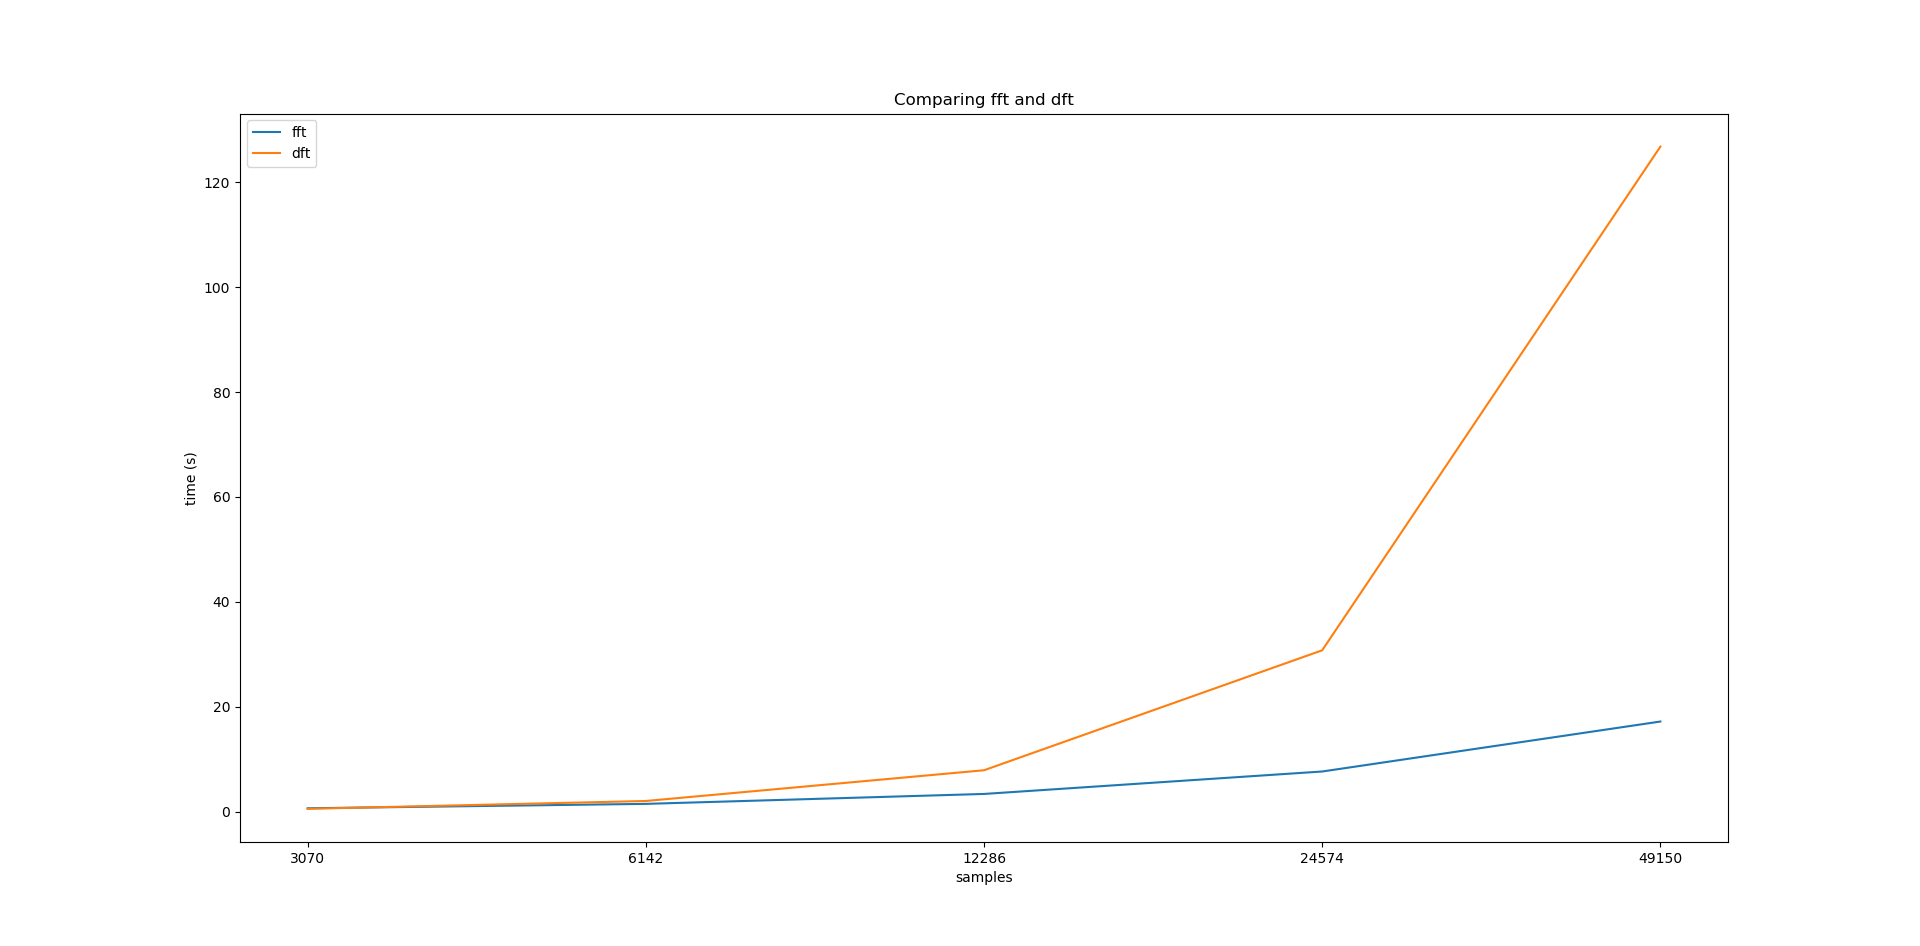
\includegraphics[width=1.4\columnwidth]{linechart_dft_vs_fft}
        \caption{A linechart of the measurements of the discrete Fourier transformation vs the fast fourier transformation.}
    \end{figure}

    \begin{figure}[h]
        \centering
        \begin{tabular}{|l|l|l|}
            \hline
            samples & DFT (s) & FFT (s) \\ \hline
            3070    & 0.55    & 0.66    \\ \hline
            6142    & 2.05    & 1.50    \\ \hline
            12286   & 7.90    & 3.39    \\ \hline
            24574   & 30.77   & 7.67    \\ \hline
            49150   & 126.78  & 17.19   \\ \hline
        \end{tabular}
        \caption{The table displays the exact values of the measurements.}
    \end{figure}

    \subsection{Profiling}

    For profiling we ran the pipeline module using a static filterbank file a 100 times with a total of 49150 samples. The pipeline module ran and measured the time it took
    to run each method of the Asteria library. After measuring the time, we calculated the standard deviation to look if there were any outliers and after noticing no significant
    outliers, we used the mean of each method for visualizing the measurements.

    To be able to compare the efficiency of the methods, we decided to visualize both a horizontal bar chart and a pie chart for each method. By doing so, we hope to see whether
    there are any significant results that we would otherwise fail to notice. Furthermore, to see whether there are any relative changes when running different sample sizes, we
    also decided to display the bar chart for both the 3070 and 49150 samples.

    After plotting the two different bar charts we noticed that there is a significant difference between the efficiency of the different methods. Especially the discerete Fourier
    transformation is incredibly slow when compared to the fast Fourier transformation (as discussed in the previous section). Furthermore, when the sample size increases, so does the difference
    between the discrete Fourier transformation and the other methods. Besides the discrete Fourier transformation there are no significant differences between the methods for the increased sample size.

    \begin{figure}[h]
        \centering
        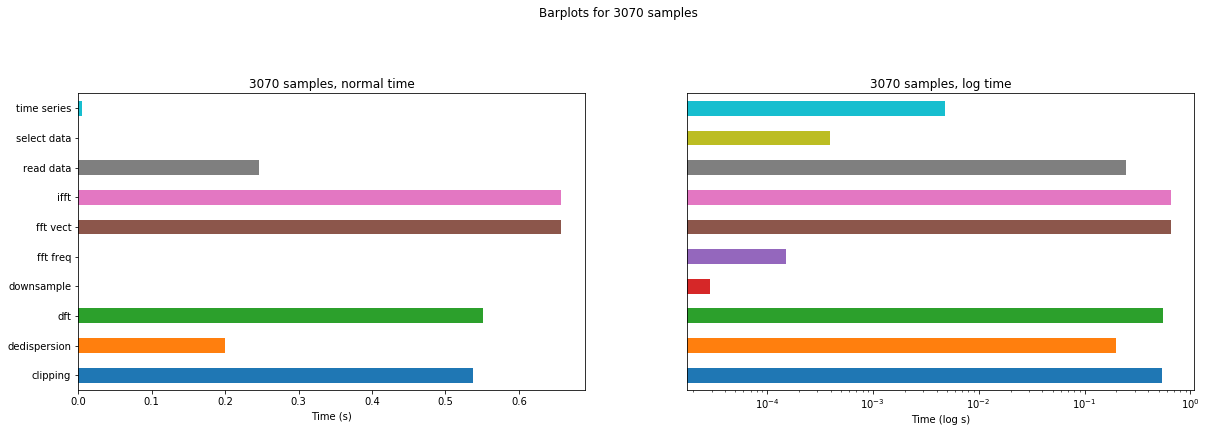
\includegraphics[width=1.2\columnwidth]{barchart_3070}
        \caption{Measured time per method for 3070 samples.}
    \end{figure}


    \begin{figure}[h]
        \centering
        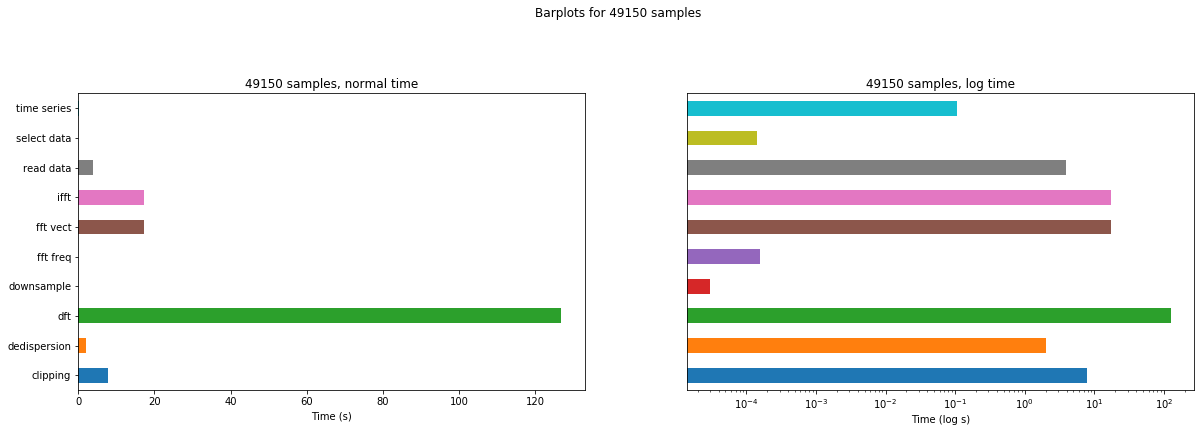
\includegraphics[width=1.2\columnwidth]{barchart_49150}
        \caption{Measured time per method for 49150 samples.}
    \end{figure}

    The results show that the average time it takes to run the entire pipeline is equal to around 175 seconds. Around 70\% of that time is spend on calculating the discrete Fourier transformations.
    After that, the fast Fourier and inverse fast Fourier transformations make up for the largest part of the remaining time, followed by the clipping module. The distribution of the time is most efficiently
    displayed using a piechart, displayed below.

    \begin{figure}[h]
        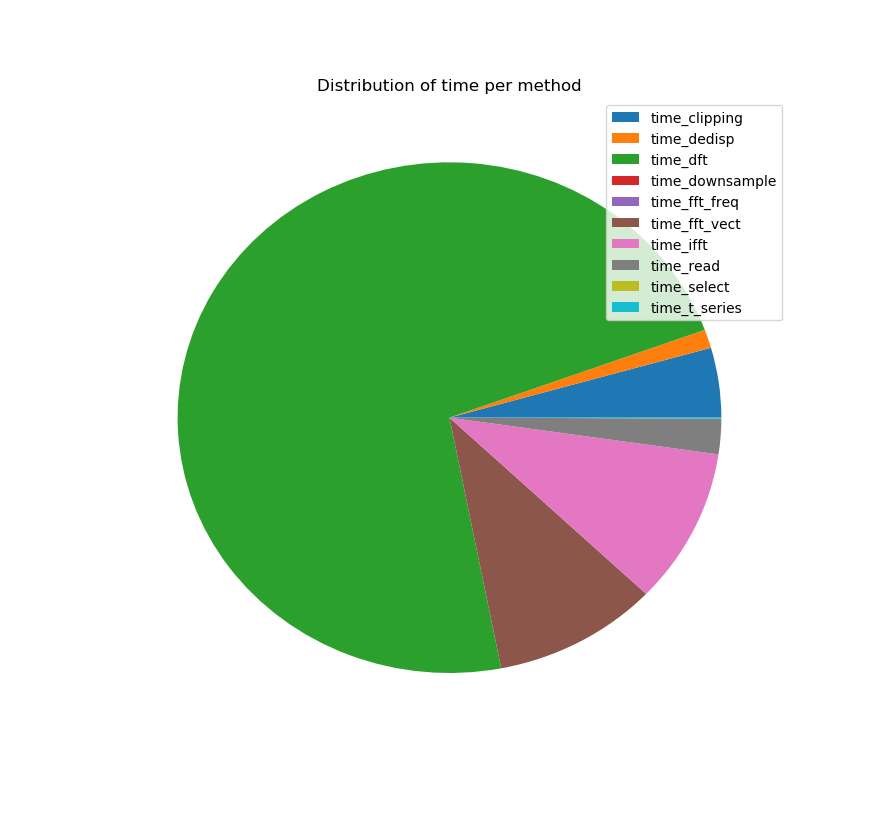
\includegraphics[width=0.9\columnwidth]{piechart_49150}
        \caption{The piechart shows how the time of running a filterbank pipeline is distributed between the different methods. }
    \end{figure}

    \end{document}